\section{GeoFit Corrections on muon \pt}
\label{sec:geofitcorr}
In CMS, the reconstructed muons can have non-zero d0 values. The effect of this residual d0 is observable as a trend in reconstructed \pt values of these muons, which in turn leads to a increase in reconstructed dimuon invariant mass resolution. This effect is corrected by \textit{GeoFit Corrections} that are derived in Z+jets MC samples and are applied to both data and MC. Fig.~\ref{fig:dimu_mass_vs_d0} shows the trend in reconstructed dimuon mass when plotted against $\text{d0}_{\mu^+}-\text{d0}_{\mu^-}$ before and after the corrections. The corrections improve the dimuon mass resolution in both data and MC without introducing an overall mass scale shift or any other bias. Fig.~\ref{fig:ggH_dimu_mass_geofit} shows dimuon mass distributions for ggH signal MC before and after the \textit{GeoFit Corrections}. The details of \textit{GeoFit Corrections} can be found in Section~\ref{sec:app_geofitcorr}.


\begin{figure}[h!]
    \centering
    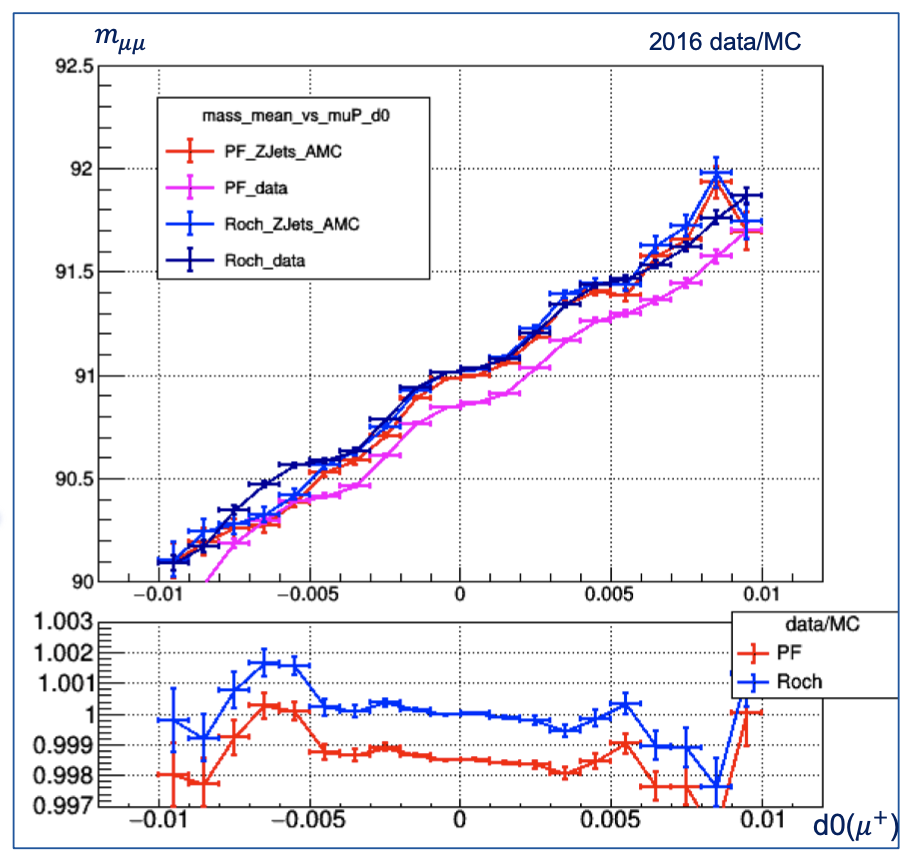
\includegraphics[width=0.49\textwidth]{images_geofit/dimu_mass_vs_d0_Roch.png}
    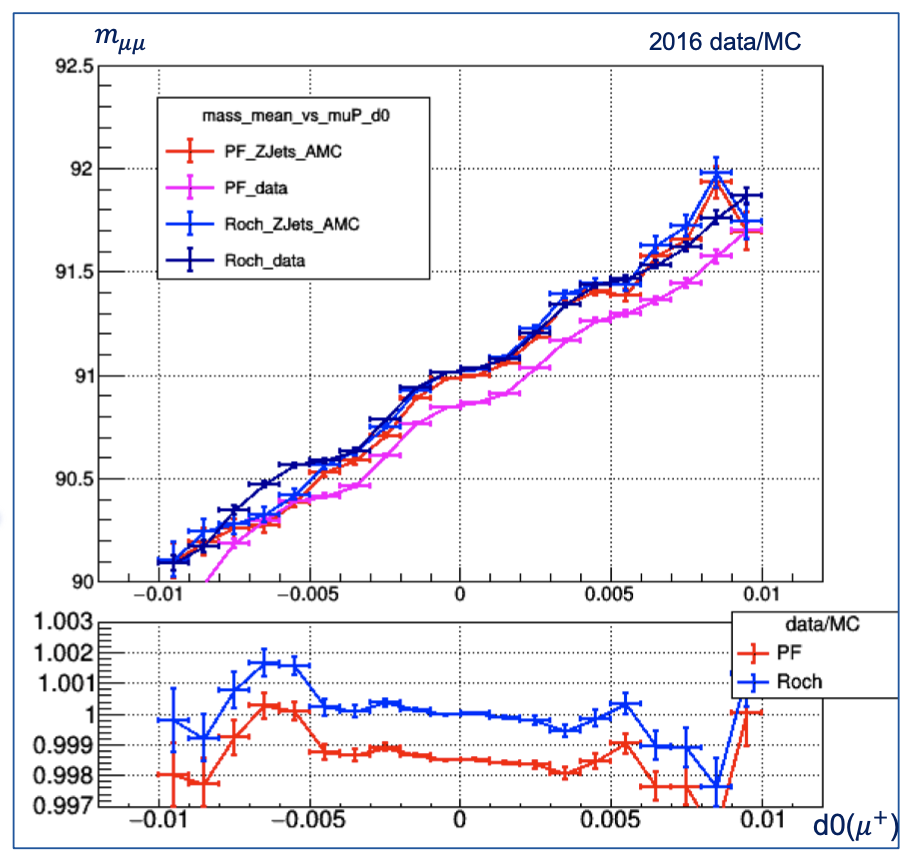
\includegraphics[width=0.49\textwidth]{images_geofit/dimu_mass_vs_d0_geofit.png}
    \caption{Dimuon mass peak mean value vs. $\text{d0}_{\mu^+}-\text{d0}_{\mu^-}$ before (left) and after (right) \textit{GeoFit Corrections} showing in 2016 Z+jets data and MC.}
    \label{fig:dimu_mass_vs_d0}
\end{figure}


\begin{figure}[h!]
    \centering
    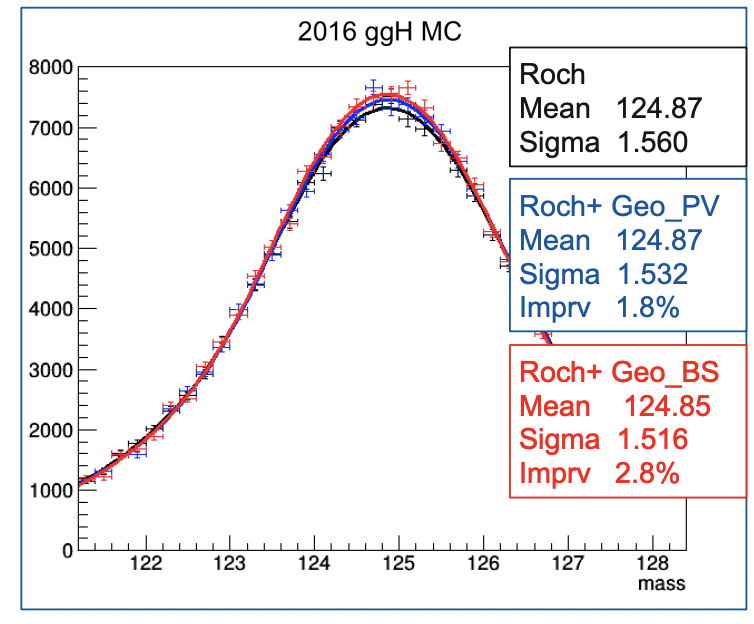
\includegraphics[width=0.32\textwidth]{images_geofit/ggH_mass_geofit_2016.png}
    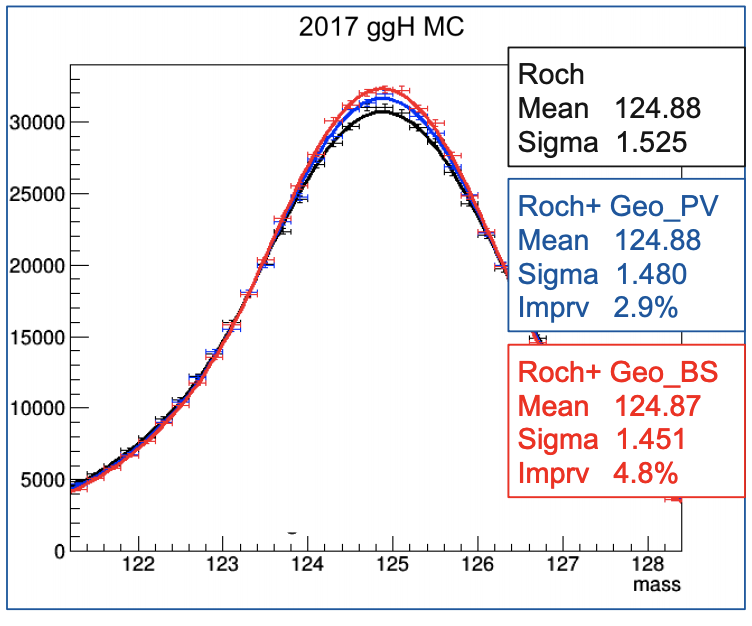
\includegraphics[width=0.32\textwidth]{images_geofit/ggH_mass_geofit_2017.png}
    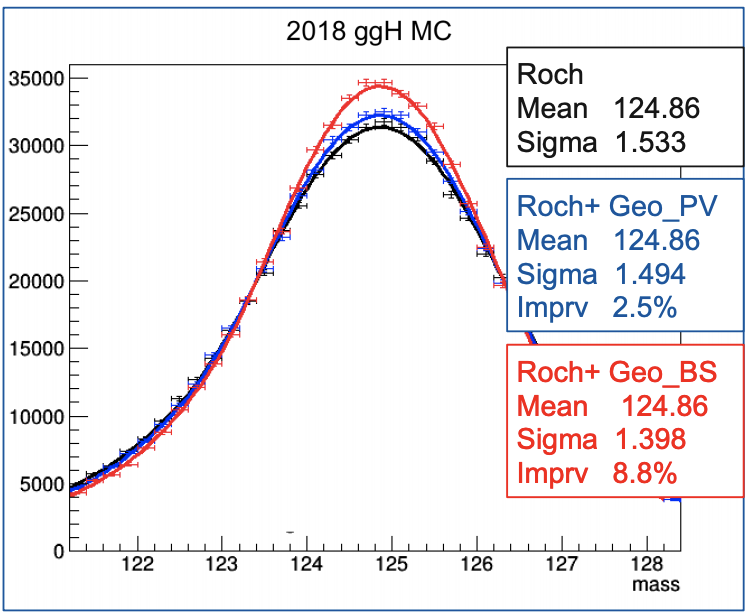
\includegraphics[width=0.32\textwidth]{images_geofit/ggH_mass_geofit_2018.png}
    \caption{Dimuon mass peak around 125 \gev for ggH signal MC samples in 2016 (left), 2017 (center) and 2018 (right) fitted by using a double-sided crystal ball function.}
    \label{fig:ggH_dimu_mass_geofit}
\end{figure}





